\documentclass{article}
\usepackage{graphicx}
\usepackage{siunitx}
\usepackage{wrapfig}

\begin{document}
    \section{Chapter 18, Problem 78}
        \begin{wrapfigure}{r}{0.35\textwidth}
            \vspace{-50pt}
            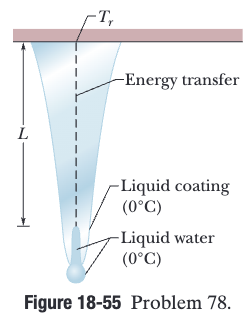
\includegraphics[width=0.35\textwidth]{picture_18-55.png} 
            % \label{fig:wrapfig}
        \end{wrapfigure}
        Icicles. Liquid water coats an active (growing) icicle and extends up a short, narrow tube along the central axis (Fig. 18-55). 
        Because the water-ice interface must have a temperature of 0\unit{\celsius}, the water in the tube cannot lose energy through the sides of the icicle or down through the tip because there is no temperature change in those directions. 
        It can lose energy and freeze only by sending energy up (through distance L) to the top of the icicle, where the temperature $T_r$ can be below 0\unit{\celsius}. 
        Take L = 0.12 m and $T_r = -5\unit{\celsius}$. 
        Assume that the central tube and the upward conduction path both have cross-sectional area A. 
        In terms of A, what rate is (a) energy conducted upward and (b) mass converted from liquid to ice at the top of the central tube? 
        (c) At what rate does the top of the tube move downward because of water freezing there? 
        The thermal conductivity of ice is 0.400 \unit{\watt/\meter\cdot\kelvin}, and the density of liquid water is 1000 \unit{\kilo\gram/\meter^3}.

    \pagebreak
    \section{Chapter 18, Problem 95}
        \begin{wrapfigure}{r}{0.35\textwidth}
            \vspace{-55pt}
            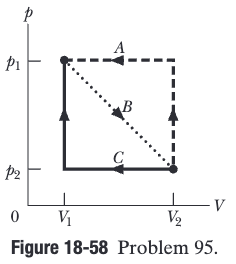
\includegraphics[width=0.35\textwidth]{picture_18-58.png} 
            % \label{fig:wrapfig}
        \end{wrapfigure}
        A sample of gas expands from $V_1 = 1.0\,\unit{\meter^3}$ and $p_1 = 40\,\unit{\pascal}$ to $V_2 = 4.0\,\unit{\meter^3}$ and $p_2 = 10\,\unit{\pascal}$ along path B in the p-V diagram in Fig. 18-58.
        It is then compressed back to $V_1$ along either path A or path C. 
        Compute the net work done by the gas for the complete cycle along (a) path $BA$ and (b) path $BC$.

        \subsection{Solution}
    
    \pagebreak
    \section{Chapter 19, Problem 35}
        Ten particles are moving with the following speeds: four at $200 \unit{\meter/\second}$, two at $500 \unit{\meter/\second}$, and four at $600 \unit{\meter/\second}$. 
        Calculate their (a) average and (b) rms speeds. 
        (c) Is $v_{rms} > v_{avg}$?

        \subsection{Solution}

    \pagebreak
    \section{Chapter 19, Problem 59}
        \begin{wrapfigure}{r}{0.35\textwidth}
            \vspace{-30pt}
            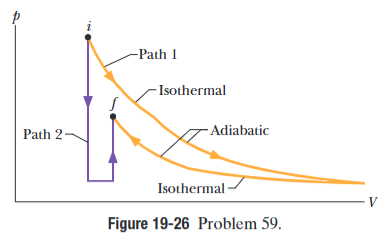
\includegraphics[width=0.35\textwidth]{picture_19-26.png} 
            % \label{fig:wrapfig}
        \end{wrapfigure}
        Figure 19-26 shows two paths that may be taken by a gas from an initial point $i$ to a final point $f$. 
        Path 1 consists of an isothermal expansion (work is 50 J in magnitude), an adiabatic expansion (work is 40 J in magnitude), an isothermal compression (work is 30 J in magnitude), and then an adiabatic compression (work is 25 J in magnitude). 
        What is the change in the internal energy of the gas if the gas goes from point $i$ to point $f$ along path 2?

        \subsection{Solution}
    
    \pagebreak
    \section{Chapter 19, Problem 71}
        The temperature of 2.00 mol of an ideal monatomic gas is raised 15.0 K in an adiabatic process. 
        What are (a) the work W done by the gas, (b) the energy transferred as heat Q, (c) the change $\Delta E_{\rm int}$ in internal energy of the gas, and (d) the change $\Delta K$ in the average kinetic energy per atom?

        \subsection{Solution}

\end{document}